\section{Introduction}
\label{sec:intro}
\hspace{1pc}Autonomous driving \cite{urmson2008autonomous} is an advanced technology that intelligent vehicles perceive road environments through onboard sensor systems, autonomously plan driving routes, and control vehicles to reach predetermined destinations. Its technical system generally includes three major parts: environmental perception, decision planning, and vehicle control \cite{amini2020learning, montemerlo2008junior}, involving multiple research fields such as computer science, mathematics, mechanical engineering, control science, and psychology \cite{chen2015deepdriving}.

However, the current autonomous driving systems still suffer from insufficient interpretability due to the existence of "black box" nature of deep learning models \cite{7979332}, greatly limiting the credibility and widespread application of various perception and decision-making methods in practical engineering. Even though the use of generative adversarial networks (GANs) \cite{zugner2020adversarial} to generate explanatory data related to decision-making has been attempted, the quality of such data is often substandard, and the training process is quite challenging. Furthermore, modern urban traffic conditions are characterized by high dynamics and strong uncertainty. When the environment is complex, the autonomous driving system may experience performance degradation. Therefore, to overcome the limitations of existing methods, there is a need to design more interpretable and robust autonomous driving systems, thereby ensuring the safety of vehicle operation.
\begin{figure}[t]
	\centering
	%\fbox{\rule{0pt}{2in} \rule{0.9\linewidth}{0pt}}
	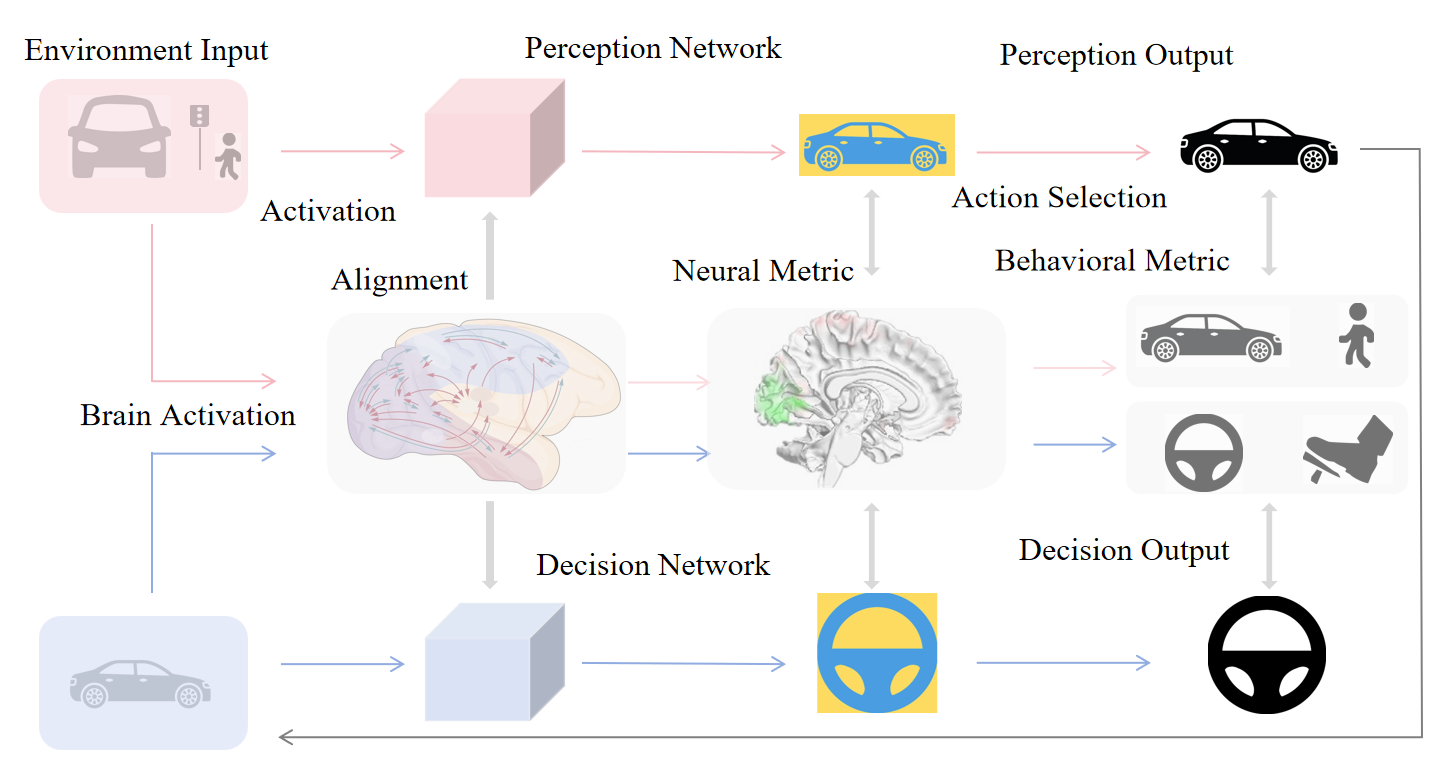
\includegraphics[width=0.8\linewidth]{brain_inspired.png}
	
	\caption{Brain-inspired Perception and Decision Network}
	\label{fig:fig1}
\end{figure}

In this paper, we propose a novel BID framework based on brain-inspired perception and decision-making. Unlike previous methods, our reinforcement learning expert does not rely on manually formulated rules and demonstrates strong interpretability and robustness. Our work involves constructing a brain-inspired perception network for extracting environmental features of the target vehicle and a brain-inspired decision-making network for generating driving decisions for the target vehicle, in order to train the reinforcement learning expert \cite{kahn2021land}. Its structure is as shown in Fig. \ref{fig:fig1}. Specifically, the brain-inspired perception network consists of a visual perception module \cite{al2018brain}, a motion perception module, and a multimodal perception module \cite{yu2023brain}. The brain-inspired decision-making network comprises a decision generation module \cite{schirner2023learning} and a decision evaluation module. Driving decisions encompass multiple driving actions of the target vehicle, and the BID agent directly imitates expert behavior. Overall, our main contribution lies in proposing a novel brain-inspired perception model and a brain-inspired decision-making model for autonomous driving, aiming to achieve a more robust and interpretable autonomous driving system.